\documentclass[aspectratio=169]{beamer}

\usepackage{subcaption}

\title{Evaluación y desarrollo de \textit{eye tracking} remoto en navegadores
\textit{web}}
\author{Francisco Figari}
\date{Buenos Aires, 2022}
\titlegraphic{
\includegraphics[width=8em]{img/logo-fcen.png}}

\setbeamertemplate{navigation symbols}{}

\setbeamertemplate{frametitle}{
  \insertsectionhead\par
  \vspace*{0.2mm}
  \insertsubsectionhead\par
  \vspace*{0.2mm}
  \insertframetitle
}

\begin{document}

\frame{\titlepage}

\section{Motivación}

\begin{frame}{~}

  \begin{itemize}
      \item Los ojos como entrada a los procesos cognitivos y estados
        emocionales de una persona
      \item Frecuentemente estudiados en el contexto de la neuropsicología
        digital para estimar el comportamiento
      \item Importante incluso cuando no son el foco del análisis
        (\textit{e.g.}, detección de caras)
      % utilizado también en el desarollo HMI, en el estudio de usabilidad de
      % interfaces, recientemente en el campo de la oftalmología para estimar
      % el campo visual
      \item Usos en otras disciplinas
  \end{itemize}

  \begin{figure}
    \begin{subfigure}{0.49\textwidth}
      \centering
      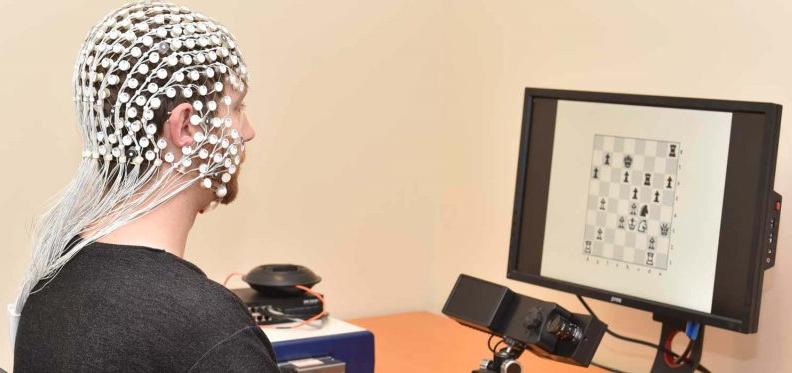
\includegraphics[width=\linewidth]{img/eye-link-eeg.jpg}
      \caption{\textit{Eye tracking} combinado con electroencefalograma}
    \end{subfigure}
    \begin{subfigure}{0.49\textwidth}
      \centering
      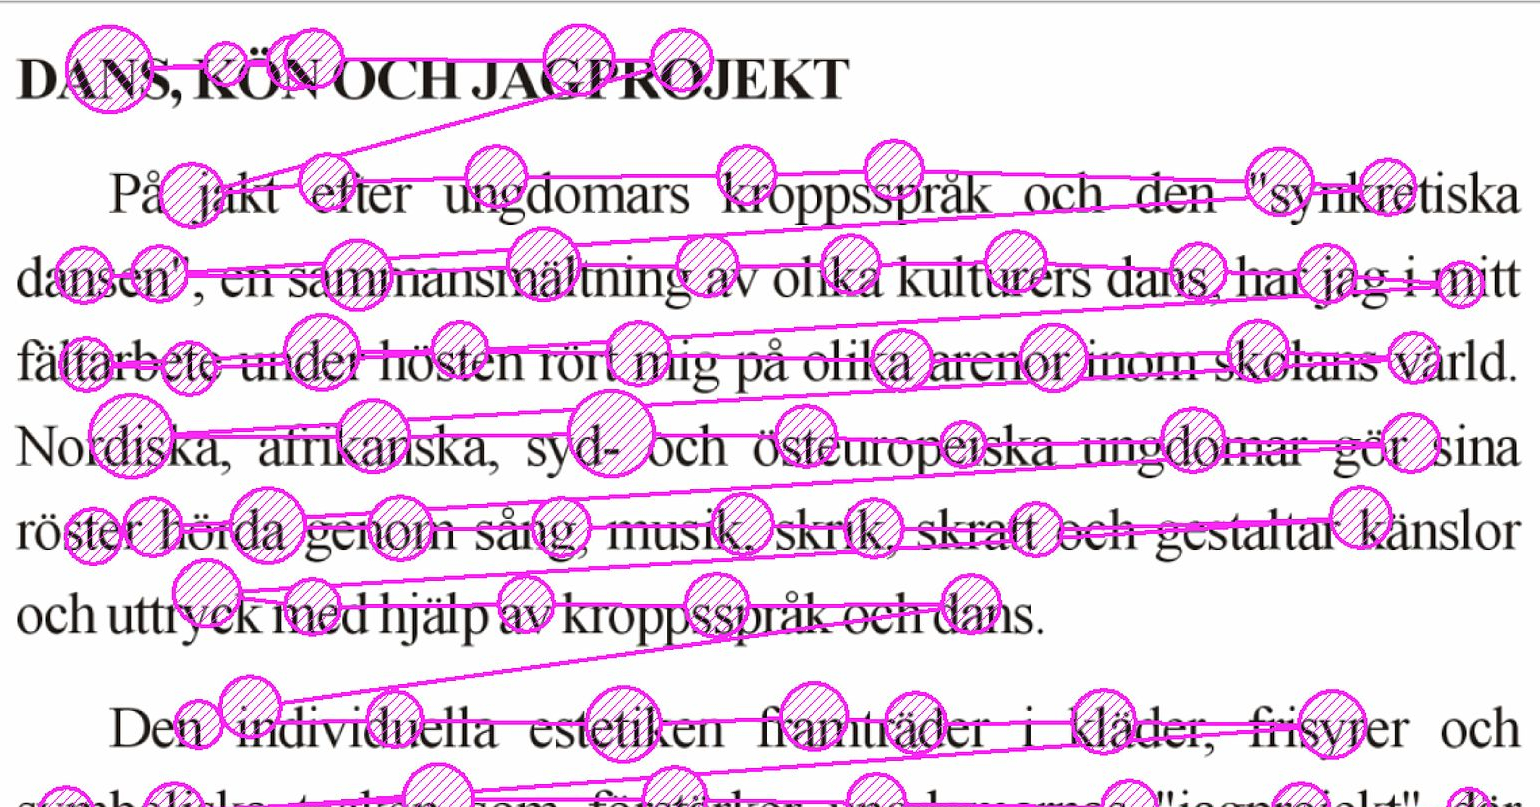
\includegraphics[width=\linewidth]{img/reading-fixations-saccades.jpg}
      \caption{Estimación de la mirada durante una tarea de lectura}
    \end{subfigure}
  \end{figure}

\end{frame}

\begin{frame}{~}

  \begin{itemize}
    \item Comunmente resuelto con sistemas comerciales cerrados
    \item Costos altos (entre 5000 y 40000 euros) mientras que el hardware en
      sí representa una pequeña fracción de estos (entre 200 y 600 euros)

    % si falta algún dato (e.g., la precisión del diámetro de la pupila) no
    % se lo puede saber
    \item Imposibilidad de auditar la implementación
    \item Necesidad de asistir a un laboratorio
  \end{itemize}

  \begin{figure}
    \begin{subfigure}{0.49\textwidth}
      \centering
      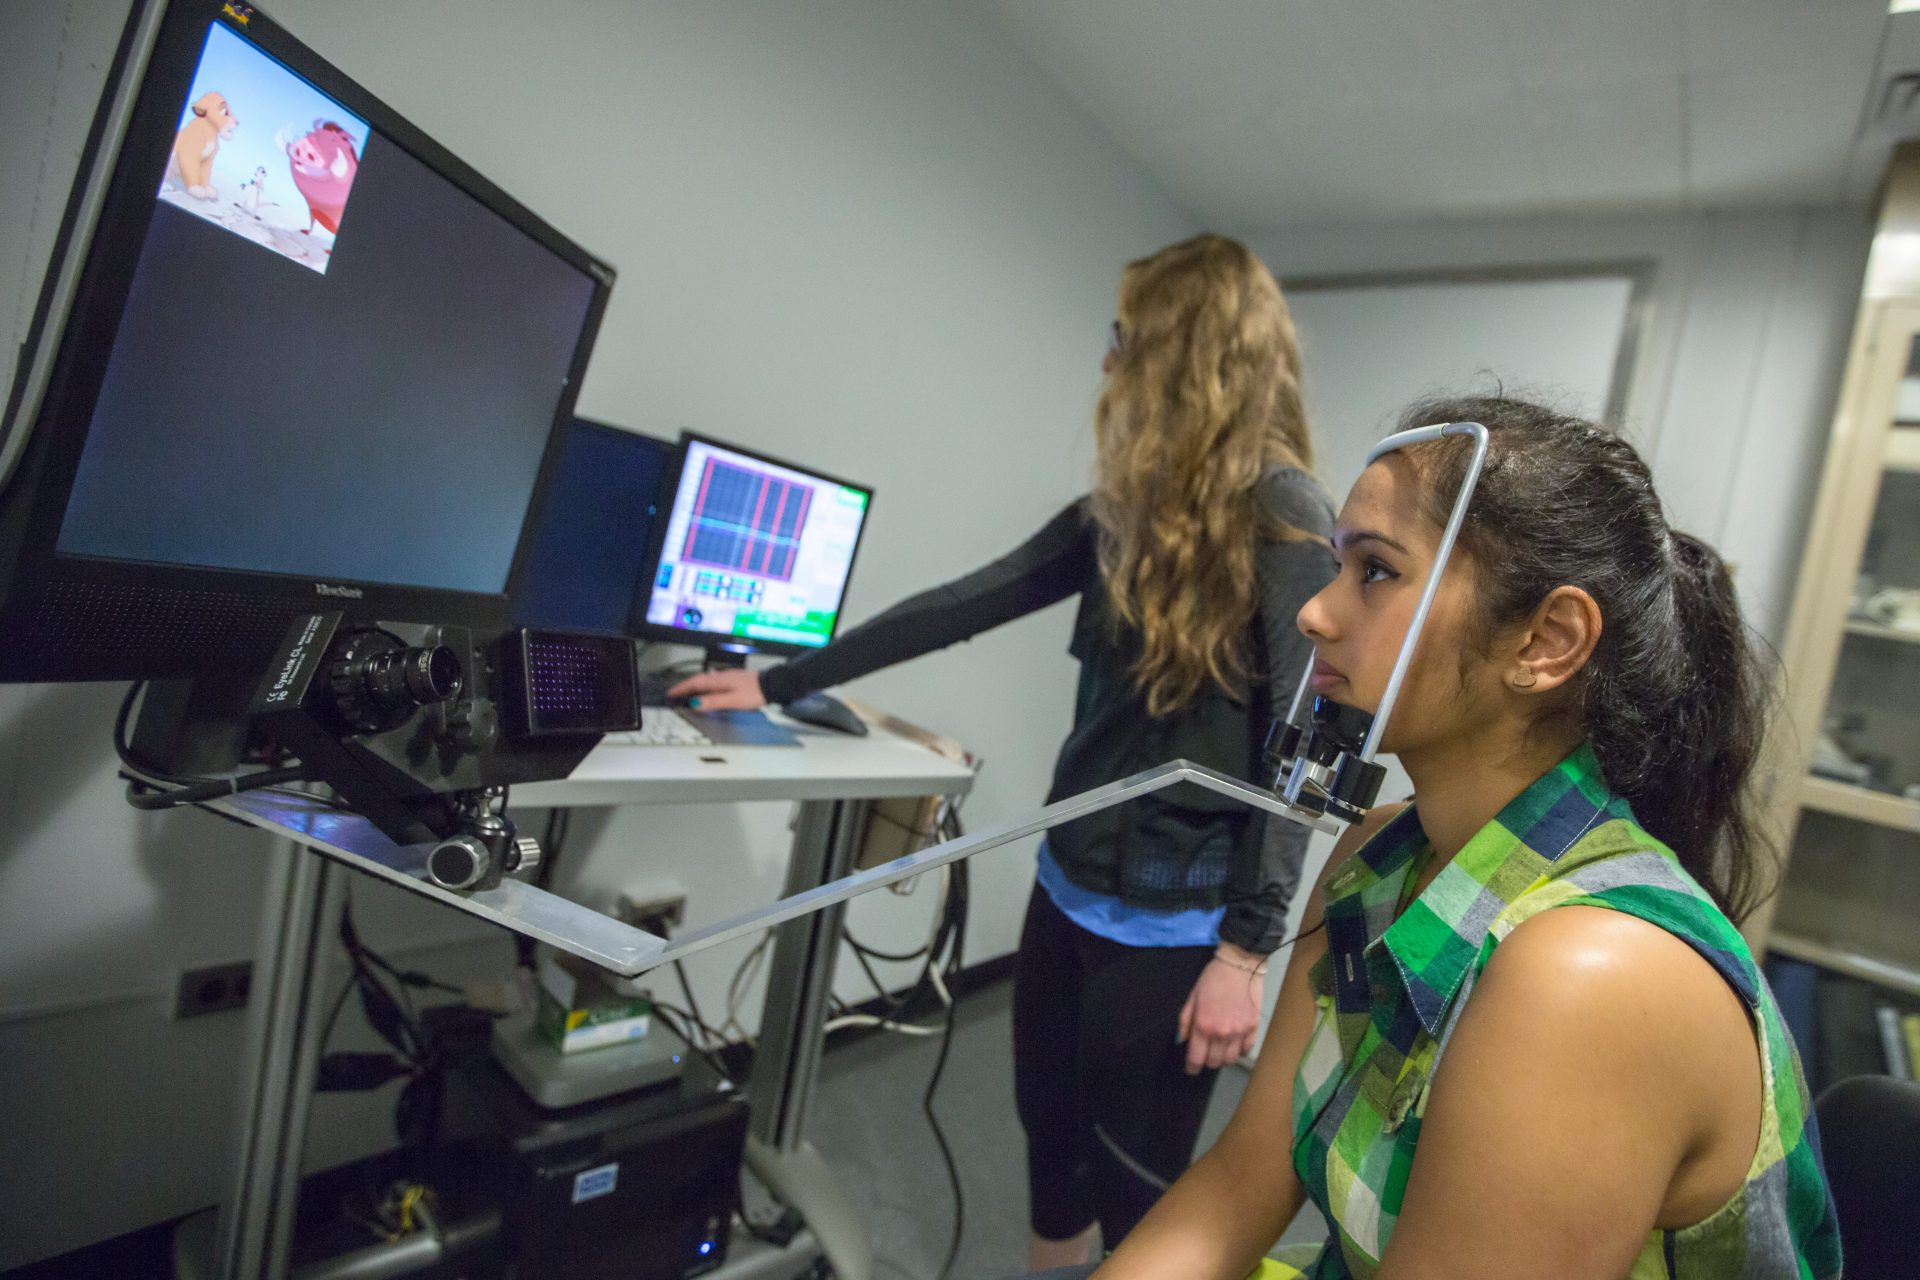
\includegraphics[width=0.6\linewidth]{img/eye-link-chinrest.jpg}
      \caption{La reestricción de movimiento facilita mantener calibrado el
      sistema}
    \end{subfigure}
    \begin{subfigure}{0.49\textwidth}
      \centering
      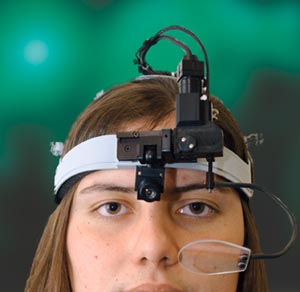
\includegraphics[width=0.5\linewidth]{img/eye-tracker-head-mounted.jpg}
      \caption{\textit{Eye tracker} montado a la cabeza}
    \end{subfigure}
  \end{figure}

\end{frame}

\begin{frame}{~}

  \begin{columns}
    \begin{column}{0.4\textwidth}
      \begin{itemize}
        \item Interés en proveer software de \textit{eye tracking}

        \item Posibilidad de \textit{crowdsourcing}

          % e.g., detectar pérdidas de atención en clases masivas
        \item Potencial para nuevas aplicaciones
      \end{itemize}

    \end{column}
    \begin{column}{0.6\textwidth}

      \begin{figure}
        \begin{subfigure}{0.49\textwidth}
          \centering
          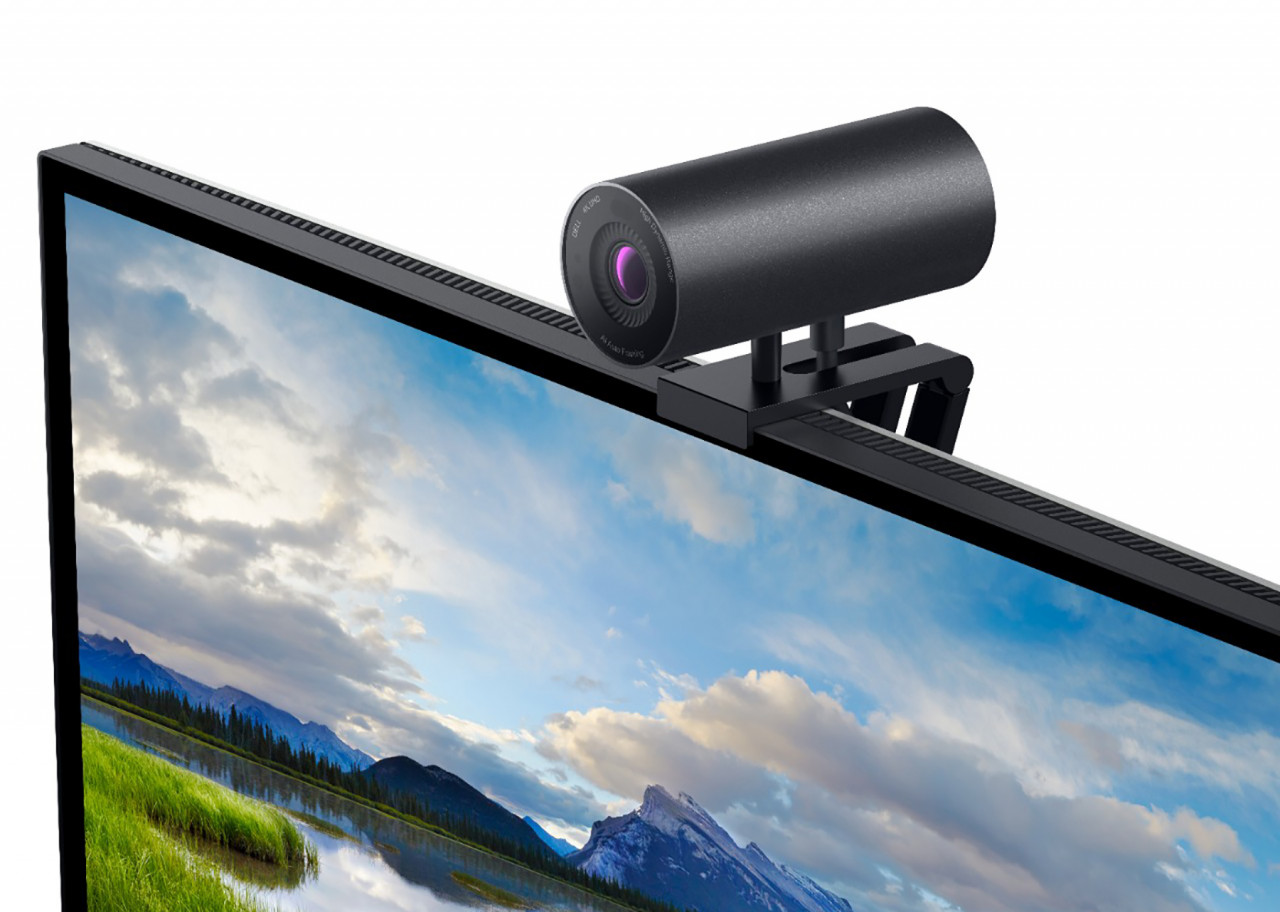
\includegraphics[width=0.8\linewidth]{img/external-webcam.jpg}
        \end{subfigure}
        \begin{subfigure}{0.49\textwidth}
          \centering
          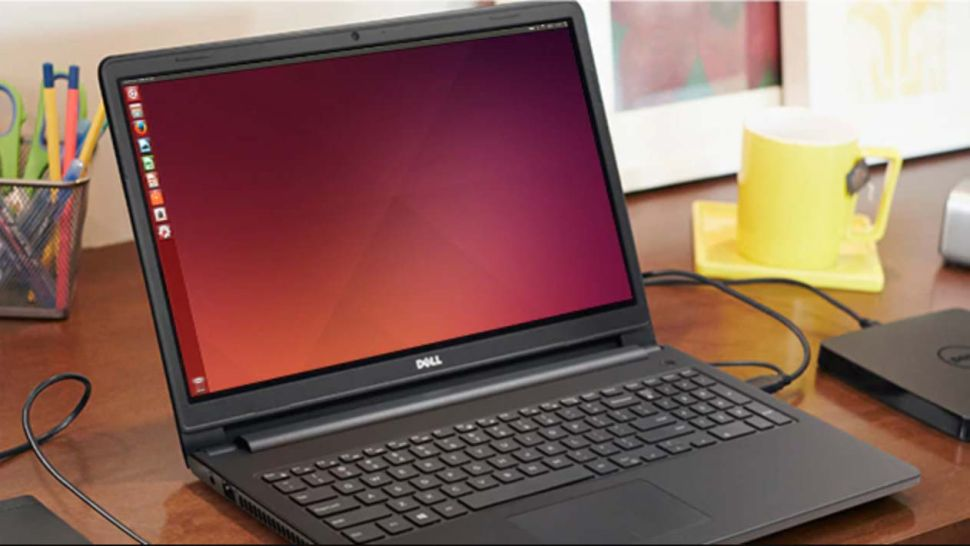
\includegraphics[width=0.8\linewidth]{img/notebook.jpg}
        \end{subfigure}
        \caption{Webcams domésticas ya disponibles}
      \end{figure}

      \begin{figure}
        \begin{subfigure}{0.49\textwidth}
          \centering
          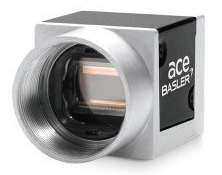
\includegraphics[width=0.6\linewidth]{img/basler-camera.jpg}
        \end{subfigure}
        \begin{subfigure}{0.49\textwidth}
          \centering
          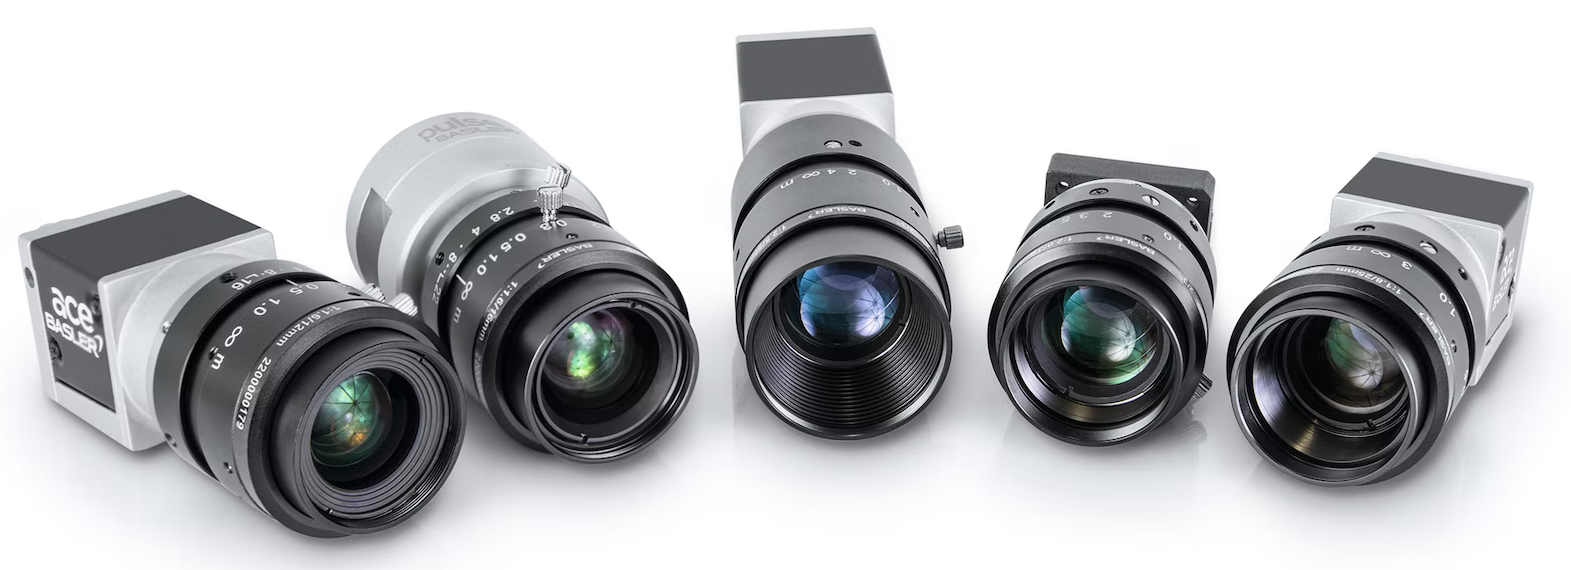
\includegraphics[width=0.8\linewidth]{img/basler-cameras-with-lens.png}
        \end{subfigure}
        \caption{Hardware profesional adquirible por una fracción del costo}
      \end{figure}


    \end{column}
  \end{columns}
\end{frame}

\section{Objetivos}

\begin{frame}{~}

  \begin{itemize}
    \item Evaluar implementaciones recientes con similares motivaciones
    % - entender el problema
    % - definir los requerimientos
    % - establecer qué puede reutilizarse

    \item Implementar un prototipo de \textit{eye tracker} que corra en
      navegadores \textit{web} y que esté orientado a análisis clínicos
    % - adaptar lo que pudiera reutilizarse
    % - implementar los módulos que faltaran

    \item Emular análisis clínicos remotos y recolectar datos utilizando el
      prototipo implementado

    \item Establecer la capacidad del prototipo en replicar conclusiones
      establecidas con \textit{eye trackers} profesionales de laboratorio

  \end{itemize}

\end{frame}

\section{Caso de estudio: tarea de antisacadas}

\begin{frame}{~}

  \begin{columns}
  \begin{column}{.5\textwidth}
    \begin{itemize}
      \item Tarea corta dónde debe \textbf{evitarse} mirar un estímulo visual
        lateral; en la tarea de prosacadas debe \textbf{mirarse} tal estímulo

      \item Variaciones sutiles en su diseño según cada trabajo
      % - qué fases, escondo el estímulo central
      % - qué tiempos uso entre fases
      % - forma y color de los estímulos

      \item Expone distintos procesos cognitivos, en distinta medida según el diseño elegido
      % - inhibición respuestas reflexivas
      % - memoria visual espacial (esto por ejemplo no entra en juego con el diseño elegido)
      % - mantenimiento de la atención en un objetivo
    \end{itemize}
  \end{column}
  \begin{column}{.5\textwidth}
    \begin{figure}
      \centering
      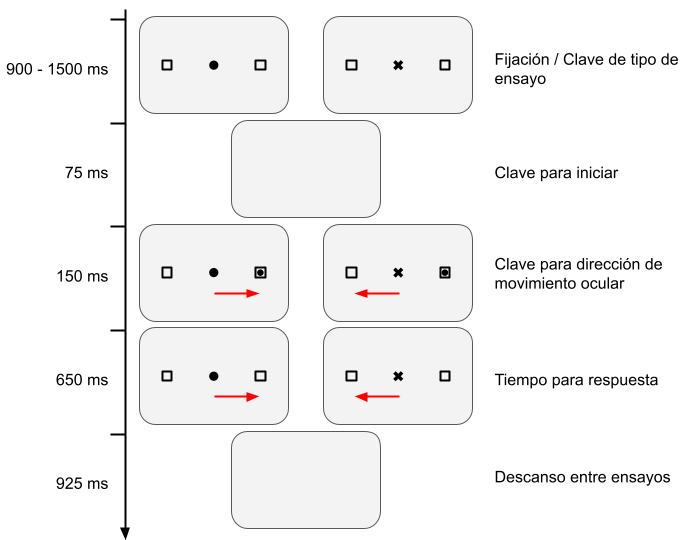
\includegraphics[width=\linewidth]{img/antisaccades-protocol.png}
      \caption{Protocolo de las tareas}
    \end{figure}
  \end{column}
  \end{columns}

\end{frame}

\begin{frame}{~}
    \begin{itemize}
    \item Resultados consistentes dentro de una misma población
    % - mayor tasa de correctitud para los casos de prosacada que para aquellos de antisacada
    % - para los grupos correctos se esperan mayores tiempos de respuesta en las repeticiones de antisacadas que en aquellas de prosacadas
    % - a mayor edad menor rendimiento en la tarea, tanto en latencia como en correctitud

    \item Búsqueda de establecer resultados para poblaciones de distinta condición neuropsicológica
    % - ditintos tipos de lesiones cerebrales
    % - déficit de atención, esquizofrenia, síndrome de Parkinson, síndrome de Tourette
    % - individuos sanos, efectos de la edad

    \item Comparación dificultosa entre distintos trabajos
    % - se obtienen valores del mismo orden (RT y correctitud) para pacientes sanos en un estudio que para pacientes con esquizofrenia de otro estudio
    \end{itemize}

\end{frame}

\section{Alternativas al \textit{eye tracking} tradicional}

\subsection{Trabajos previos}

% TODO: Separar esto en varios frames
\begin{frame}{~}

  \begin{itemize}
    \item \texttt{PupilEXT}: software para realizar pupilometría; deben
      proveerse cámaras profesionales y emisores de luz infrarroja; TODO:
      imagen pupilometría

    % hay que resaltar la importancia de esto de analizar el momento de mayor
    % coincidencia
    \item \texttt{PACE}: aplicación de escritorio basada en webcam; calibran en
      base a interacciones del usuario; analizar el momento de mayor
      coincidencia entre la mirada y la posición de la interacción; TODO:
      alguna imagen del paper

    \item \texttt{TurkerGaze}: aplicación web basada en webcam; generación de
      mapas de saliencia a través de \textit{crowdsourcing}; TODO: imagen mapas
      de saliencia

    \item \texttt{WebGazer}: aplicación web basada en webcam; se basan en
      \texttt{PACE} y \texttt{TurkerGaze}; provisto en forma de paquete; TODO:
      screenshot del paquete

  \end{itemize}

\end{frame}

\subsection{Implicancias del contexto remoto de navegador \textit{web}}

\begin{frame}{~}

  \begin{itemize}
    \item[+] Posibilidad de reutilizar cámaras web

    \item[+] Compatibilidad con otras herramientas web, en particular
      \texttt{JSPsych}

    % no es el fin del mundo pero es un lenguaje bastante odiado e implica
    % dificultades en cuanto a la precisión. Por ejemplo, la duración de cada
    % frame va a ser variable, lo que dificulta mostrar estímulos durante
    % cortas cantidades de tiempo
    \item Necesidad de implementar sobre JavaScript

    % no sólo las webcams son variables si no que tmb la compu donde corre el 
    % programa
    \item[--] Hardware variable de potencialmente bajo rendimiento

    % deben transmitirse en texto e imagenes sin que puedan hacerse
    % aclaraciones en el momento. esto implica una duración total del
    % experimento potencialmente mayor
    \item[--] Las instrucciones no pueden ser transmitidas en persona

    % puede variar la luz o la disposición del hardware
    \item[--] Ambiente físico no controlado
  \end{itemize}

  TODO: Screenshots de JSPsych y de Amazon Mechanical Turk

\end{frame}

\subsection{Modelado de la mirada}

\begin{frame}{~}
  \begin{itemize}
    % no entrar en detalle con esto pero mencionar brevemente por qué
    \item Limitados a una pequeña fracción de la bibliografía debido a tener
      una y sólo una cámara
    
    % acuerdo en que hay que mostar una serie de puntos pero no está claro
    % cuántos, ni cómo, ni qué información rescatar. tmb hay interés en
    % minimizar la duración del exp
    \item Falta de estándar respecto de cómo calibrar

    % ante ligeros movimientos de cabeza el sistema va a quedar descalibrado.
    % hay que tenerlo en cuenta en el flow del experimento. puede recalibrarse
    % cada un tiempo fijo (TG), agregar data de calibración a medida que avanza
    % el experimento (WG) o bien implementarse alguna heurística para decidir
    % cuándo el sistema necesita una recalibración
    \item Ausencia de invarianza frente a movimientos de cabeza y de
      reestricción de movimiento
  \end{itemize}
\end{frame}

\section{Implementación}

\subsection{\texttt{WebGazer} como punto de partida}

\begin{frame}{~}

  \begin{columns}
    \begin{column}{.4\textwidth}
      \begin{itemize}
        \item[+] Extracción de frames a través de la API del navegador
        \item[+] Modelos de localización de los ojos y de estimación de la
          mirada
        \item[--] Calibración inadecuada
        \item[--] Ausencia de notificación de descalibraciones
      \end{itemize}
    \end{column}

    \begin{column}{.6\textwidth}
      \begin{figure}
        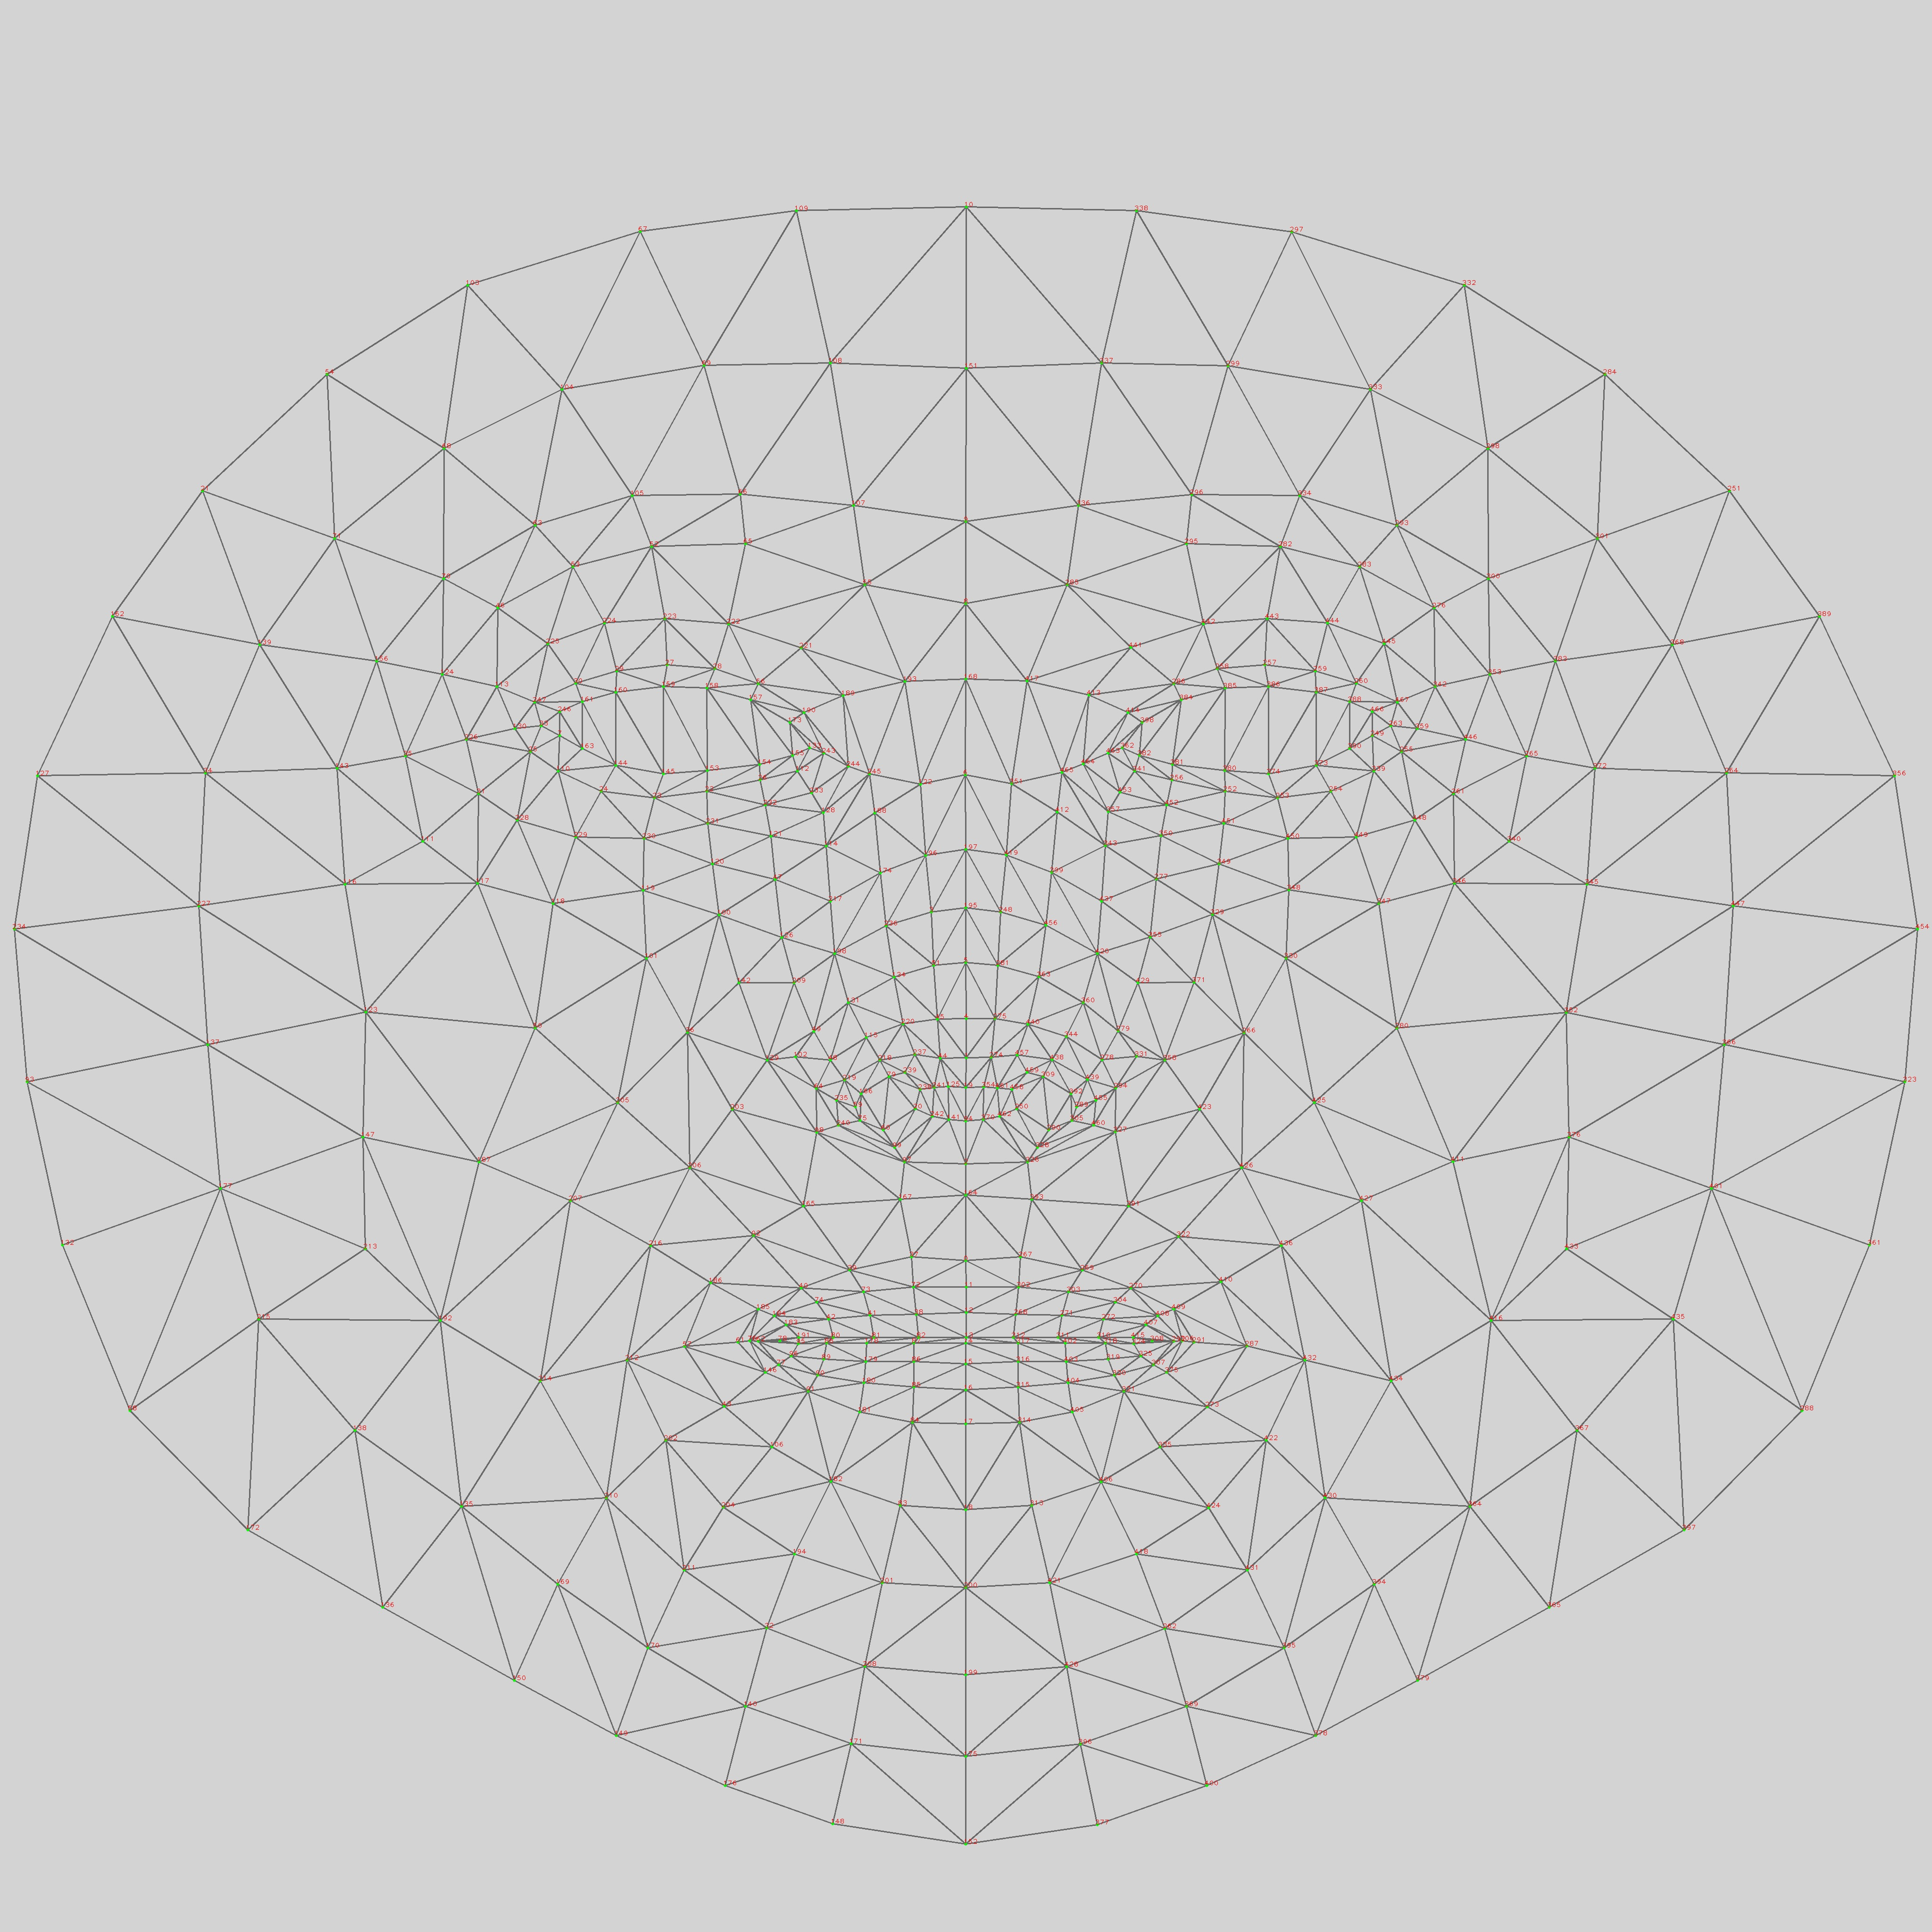
\includegraphics[width=0.6\linewidth]{img/facemesh-kepyoints.jpg}
        \caption{\textit{Output} del modelo de \textit{facemesh} utilizado por
        \texttt{WebGazer} para la localización de los ojos}
      \end{figure}
    \end{column}
  \end{columns}

\end{frame}

\subsection{Calibración y validación}

\begin{frame}{~}
  \begin{itemize}
    % La calibración de WG asume que el usuario va a estar haciendo clicks o 
    % moviendo el mouse. Siguiendo las líneas de PACE, cuando uno realiza estas
    % acciones se asume que el sujeto está mirando al puntero, utilizando esto
    % como nuevos datos de calibración
    \item Nuestro caso de uso no garantiza interacciones

    \item Se muestran una serie de puntos, para cada uno de los cuales el
      usuario tendrá que fijar la mirada y presionar la barra de espacio; TODO:
      un diagrama que muestre las posiciones de los puntos
    
    \item Validación post calibración implementada de similar manera

    \item Optimización sobre \texttt{WebGazer} en base a estas diferencias en
      la calibración
  \end{itemize}
\end{frame}

\subsection{Descalibración}

\begin{frame}{~}

  \begin{columns}
    \begin{column}{.5\textwidth}
      TODO: Pseudocódigo instanciación al finalizar la calibración \par
      TODO: Pseudocódigo del chequeo en cada frame
    \end{column}

    \begin{column}{.5\textwidth}
      TODO: Screenshot del playground de la región válida
    \end{column}
  \end{columns}

\end{frame}

\subsection{Interfaces lógicas}

\begin{frame}{~}
  \begin{columns}
    \begin{column}{.5\textwidth}
      \begin{itemize}
        \item División explícita entre el código propio del \textit{eye
          tracker} y aquel de la interfaz \texttt{JSPsych}

          % Esto evita acoplamiento del código y facilita el desarrollo
        \item Un \textit{playground} para cada interfaz
      \end{itemize}
    \end{column}

    \begin{column}{.5\textwidth}
      TODO: Par de screenshots de los playgrounds
    \end{column}
  \end{columns}

\end{frame}

\section{Experimentación}

\begin{frame}{~}
  \begin{columns}
    \begin{column}{0.5\textwidth}
      Primera instancia:
      \begin{itemize}
        \item Limitados a 10 minutos debido a una falla de \texttt{WebGazer}
        \item Únicamente ensayos de antisacada
        \item Recalibración luego de cada notificación de descalibración
        \item Sin validación post calibración
      \end{itemize}
    \end{column}
    \begin{column}{0.5\textwidth}
      Segunda instancia:
      \begin{itemize}
        \item Duración superior a 20 minutos
        \item Ensayos de prosacadas y de antisacadas

        % esto es un poco más similar a lo que hace TG
        % tmb queda en duda en qué punto es útil la notificación de
        % descalibración, porque no se estudió cómo evoluciona la calidad de
        % las estimaciones, TODO: esto en trabajo futuro capaz tenga más
        % sentido mencionarlo
        \item Recalibración cada 10 ensayos y sólo si se detectó una
          descalibración
        \item Con validación post calibración
      \end{itemize}
    \end{column}
  \end{columns}

  TODO: Screenshots JSPsych, Cognition y NeuroPruebas
\end{frame}

\section{Resultados}

\subsection{Características de los datos}

\begin{frame}{Frecuencias de muestreo}

  TODO: Acomodar subplots
  \begin{figure}
    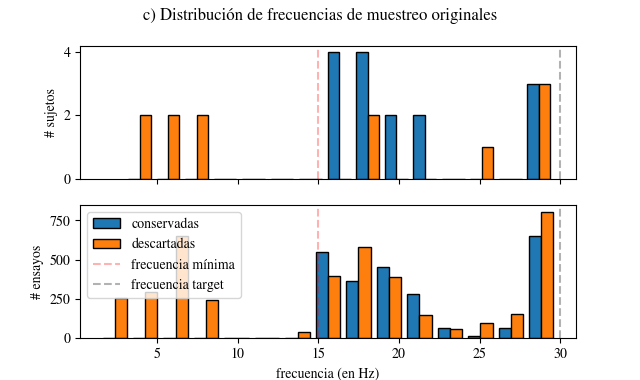
\includegraphics[width=0.7\linewidth]{img/second-sampling-frequencies-distribution.png}
  \end{figure}

\end{frame}

\begin{frame}{Anchos de pantalla}

  TODO: Acomodar subplots
  \begin{figure}
    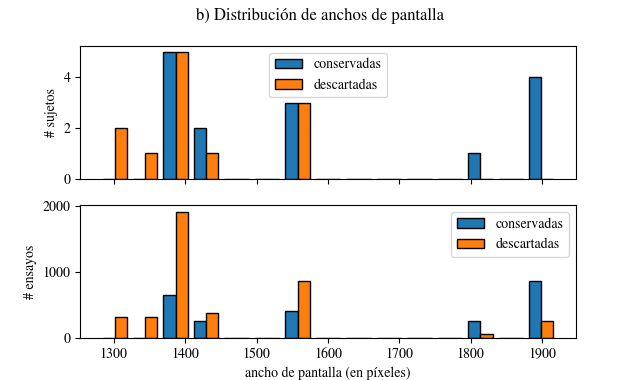
\includegraphics[width=0.7\linewidth]{img/second-widths-distribution.png}
  \end{figure}

\end{frame}

\begin{frame}{Estimaciones desviadas}

  TODO: Acomodar subplots
  \begin{figure}
    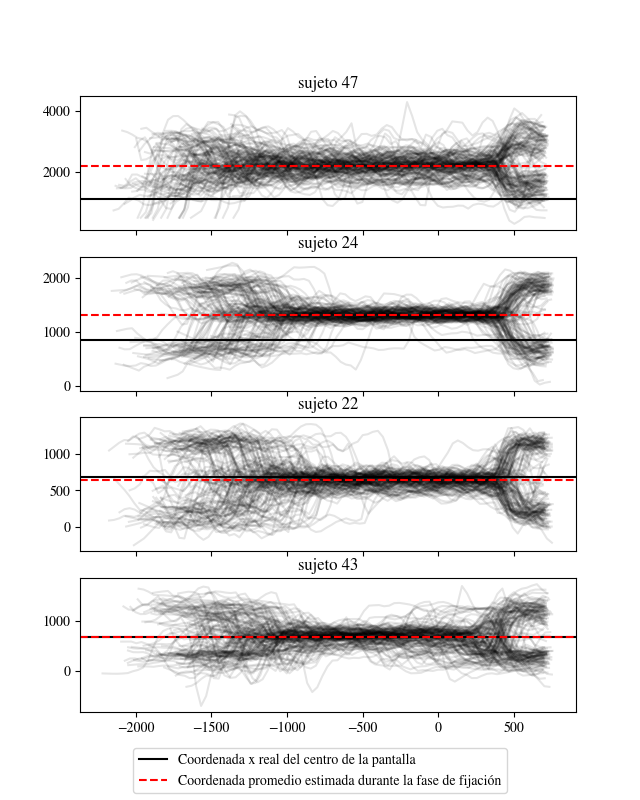
\includegraphics[width=0.8\linewidth]{img/skewed-estimations-examples.png}
  \end{figure}

\end{frame}

\subsection{Limpieza y normalización}

% No hacer mucho hincapié acá y comentar que en cualquier caso está disponible
% la implementación
\begin{frame}{~}

  \begin{columns}
    \begin{column}{0.5\textwidth}
      TODO: Ejemplo de la interpolación de estimaciones
      TODO: Ejemplo de datos descartados
    \end{column}
    \begin{column}{0.5\textwidth}
      \begin{figure}
        \centering
        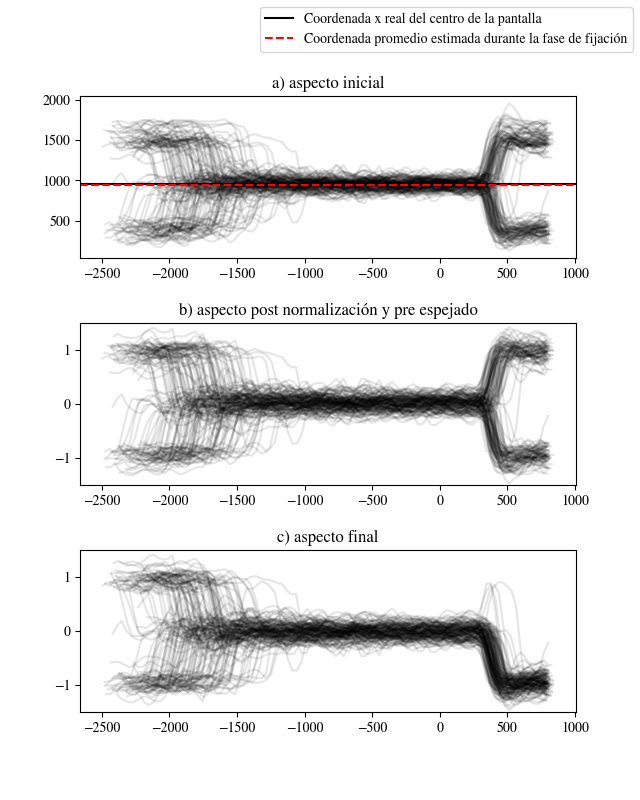
\includegraphics[width=\linewidth]{img/normalization-looks-example.png}
      \end{figure}
    \end{column}
  \end{columns}

\end{frame}

\subsection{Detección de sacadas}

\begin{frame}{~}

  Luego de normalizar, se considerará un intervalo como una sacada si:
  \begin{enumerate}
    \item La mirada se mueve en una misma dirección
    \item El intervalo dura al menos 40 ms
    \item Se recorre \textit{cierta} distancia mínima durante ese intervalo
    \item El desplazamiento es lo \textit{suficientemente rápido}
  \end{enumerate}
  Implementación \textit{ad hoc} cuya calidad no fue estudiada.

\end{frame}

\subsection{Conclusiones generales replicados}

\begin{frame}{~}
TODO: tablas
\end{frame}

\subsection{Menos datos de lo esperado}

\begin{frame}{~}
  \begin{columns}
    \begin{column}{0.4\textwidth}
      \begin{itemize}
        \item Descarte de aproximadamente $\frac{2}{3}$ de los datos
        \item Nula representatividad de sujetos de edad mayor a 50 años
        \item Baja representatividad por sujeto del grupo incorrecto
      \end{itemize}
    \end{column}

    \begin{column}{0.6\textwidth}
      \begin{figure}
        \centering
        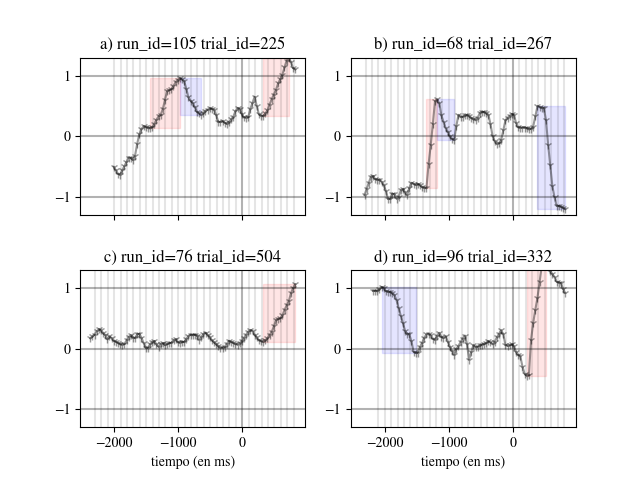
\includegraphics[width=0.9\linewidth]{img/undetected-saccades-examples.png}
      \end{figure}
    \end{column}
  \end{columns}
\end{frame}

\section{Conclusiones}

\begin{frame}{~}
. qué se obtuvo
. potencial para realizar análisis clínicos pero muy verde y muy por debajo de
  la precisión alcanzable con et profesionales
. protocolo de utilización
\end{frame}

% TODO: Las limitaciones y trabajo futuro no ponerlas todas y en cambio referir
% a la tesis
\subsection{Limitaciones}

\begin{frame}{Implementativas}
. bajas frecuencias
. pestañeos
. estimación del tamaño de la pantalla
. imprecisión en la duración de cada frame, problemático si se quiere mostrar
  un estímulo durante una corta duración de tiempo
\end{frame}

\begin{frame}{Experimentales}
. proporción de datos filtrados demasiado elevada
. necesidad de revisar la causa de las altas tasas de correctitud obtenidas
. representatividad de distintos grupos etarios
\end{frame}

\subsection{Trabajo futuro}

\begin{frame}{Análisis de datos}
. Investigar e implementar mecanismos estándares de detección de sacadas, lo
  cual podría basarse en la previa construcción de un dataset etiquetado de
  sacadas
. Revisar criterios de exclusión para asegurarse de no estar filtrando datos
  válidos
. Realizar nuevas rondas de experimentación, estimando previamente la cantidad
  de ensayos necesarios para asegurar cantidades suficientes en los grupos
  incorrectos y en los distintos grupos etarios
\end{frame}

\begin{frame}{Análisis de sensibilidad}
. propuesta sobre experimento para recolectar datos y establecer métricas de
  calidad sobre las estimaciones obtenidas por la herramienta
TODO: Acá combinar un poco lo que quedó en la tesis y lo que pensé para
      sensitivity analysis
\end{frame}

\begin{frame}{Prototipo desarrollado}
. optimizar frecuencia de muestreo
. reexplorar detección de descalibraciones y qué significa que el sistema esté
  descalibrado
. mejorar la calibración, generalizarla a más puntos de interés
. detección de pestañeos
. estimación del tamaño de la pantalla y posibilidad de mostrar estímulos en
  grados
. verificación de condiciones iniciales
TODO: Extender con lo que haya escrito en la tesis
\end{frame}

\begin{frame}{\textit{Eye tracking} en navegadores \textit{web}}
. extender bibliografía que aplique a nuestro contexto
. eye tracking web no podría atacar algunos problemas que sí puede el eye
  tracking tradicional, pero al ser remoto y de bajo costo es posible que
  permita atacar nuevos problemas. Deben entonces buscarse tales problemas
\end{frame}

\end{document}
